\documentclass[11pt]{article}

\usepackage{graphicx}
\usepackage{amssymb}
\usepackage{amsmath}
\usepackage[left = 2cm, right = 2cm, top = 2cm, bottom = 2cm]{geometry}
\usepackage{hyperref}
\usepackage{xcolor}
\usepackage{physics}
\usepackage{soul}
\usepackage{subcaption}

\definecolor{red2}{RGB}{255, 49, 49}
\definecolor{green2}{RGB}{144, 238, 144}
\definecolor{purple2}{RGB}{150, 111, 214}
\newcommand{\hlyellow}[1]{{\sethlcolor{yellow}\hl{#1}}}
\newcommand{\hlgreen}[1]{{\sethlcolor{green2}\hl{#1}}}
\newcommand{\hlred}[1]{{\sethlcolor{red2}\hl{#1}}}
\newcommand{\hlpurple}[1]{{\sethlcolor{purple2}\hl{#1}}}

\bibliographystyle{unsrt}%abbrv} % We choose the "plain" reference style

\title{Tips/Tricks and Notes to Simulation Tools}
\author{Danush Shekar}
\date{\today}

\begin{document}

\maketitle
\tableofcontents

\newpage

\abstract{This is my attempt in saving an account of all tips/tricks, notes, and discussions of the simulation tools I have used (mostly related to HEP simulations). In theory, this is also a note to questions and answers I encountered while I studied the subject, and that this notebook should serve as a reference for the doubts my mind stumbles upon in the future.}

\subsection*{Colour legend}
This note will follow a highlighting scheme where text highlighted in different colors mean the following:
\newline
\hlyellow{Yellow coloured text} - Doubts, or sentences that are to be clarified/understood later.\\
\hlgreen{Green coloured text} - Some takeaways.\\
%\hlred{Red coloured text} - Mistakes/typos.\\
\hlpurple{Purple coloured text} - Interesting and unique points, that often are not mentioned explicitly in textbooks/literature.\\

\section{About}
The WeightField\footnote{The manual for this (first) version can be found at \href{http://personalpages.to.infn.it/~cartigli/Weightfield2/Manual_files/Manual_Weightfield.pdf}{here}} (WF) software is a tool used to simulate a variety of silicon detectors: different versions have been updated over time to study a variety of silicon sensors. As the name suggest, the WeightField2\footnote{Main link to manuals/guides - \href{http://personalpages.to.infn.it/~cartigli/Weightfield2/Manual.html}{http://personalpages.to.infn.it/~cartigli/Weightfield2/Manual.html}.} (WF2) software is the second iteration of WF. The weighting potential is calculated by solving for the Laplace equation using numerical methods (which also involves interpolation), and the induced current is calculated using the Shockley-Ramo theorem. An important piece of information that you probably should keep at the back of your head is that ``the backplane is at the bottom and the strips on the top edge with the readout strip being always centered".

WF2-RSD (WF2 - Resistive Silicon Detectors) is a version of software that rolled-out after WF2. The primary objective of this tool is to simulate RSDs (or also known as AC-LGADs). In some parts of the code, I believe (and this is a personal opinion) that quantities being calculated are mimicing the experimental results and not truly simulating the physics behind such processes. This might also partly be because we still don't know what is happening in AC-LGADs, for example, the signal induction to the AC pads.
\newline
Two references that explain some working principles of WF2-RSD are \cite{wf2-rsd-working-principles} and \cite{Tornago2021}. The former discusses the models used to calculate the charge sharing (among different pads) and signal delay and the later is a more detailed article on the same.
\newline
WF2-RSD differs from WF2 in the following aspects:
\begin{enumerate}
    \item Resistive layer - capability to simulate a resistive layer with a user-defined resistivity.
    \item Addition of circular pads (instead of strips) by default - User can change number of pads, and packing (square and hexagonal packing of the pads).
    \item Naturally, the signal induction calculation has been updated, and the signal sharing model (Logarithmic attenuation model \cite{Tornago2021}) has been included.
\end{enumerate}

\section{Input Panel Variables/Quantities}
The WF2-RSD front-end has many parameters and sections for plots and an example of the same can be seen in Figure \ref{fig:3x3-pad-field}. This section walks the reader through what each section is for, along with a brief description of the quantities/results involved.
\subsection{Panel: Detector properties}
There are 3 detector types under the ``\textbf{Type}'' section (namely Silicon, diamond, and SiC). This refers to the type of material the detector is made of. Each option would involve different values for quanitities like dielectric constant, (e/h) mobilities, etc.
\newline
Since we are dealing with AC-LGADs, the next section ``\textbf{}'' would/should stay at n-type strips (referring to the n+ layer) and p-type bulk.
\newline
The options involved with the ``\textbf{Dimensions}" section and their description are as follows:
\begin{enumerate}
    \item Stacked - Switching-on this option will go from rectangularly packed pads (default) to hexagonal packing of the pads.
    \item Number of pads - The number of pads that will be present in the sensor geometry. A screenshot of the simulation window/screen for 2 different pad numbers are shown in Figure \ref{fig:ss-number-of-pads}.
    \begin{figure*}[h!]
        \centering
        \begin{subfigure}[t]{0.99\textwidth}
            \centering
            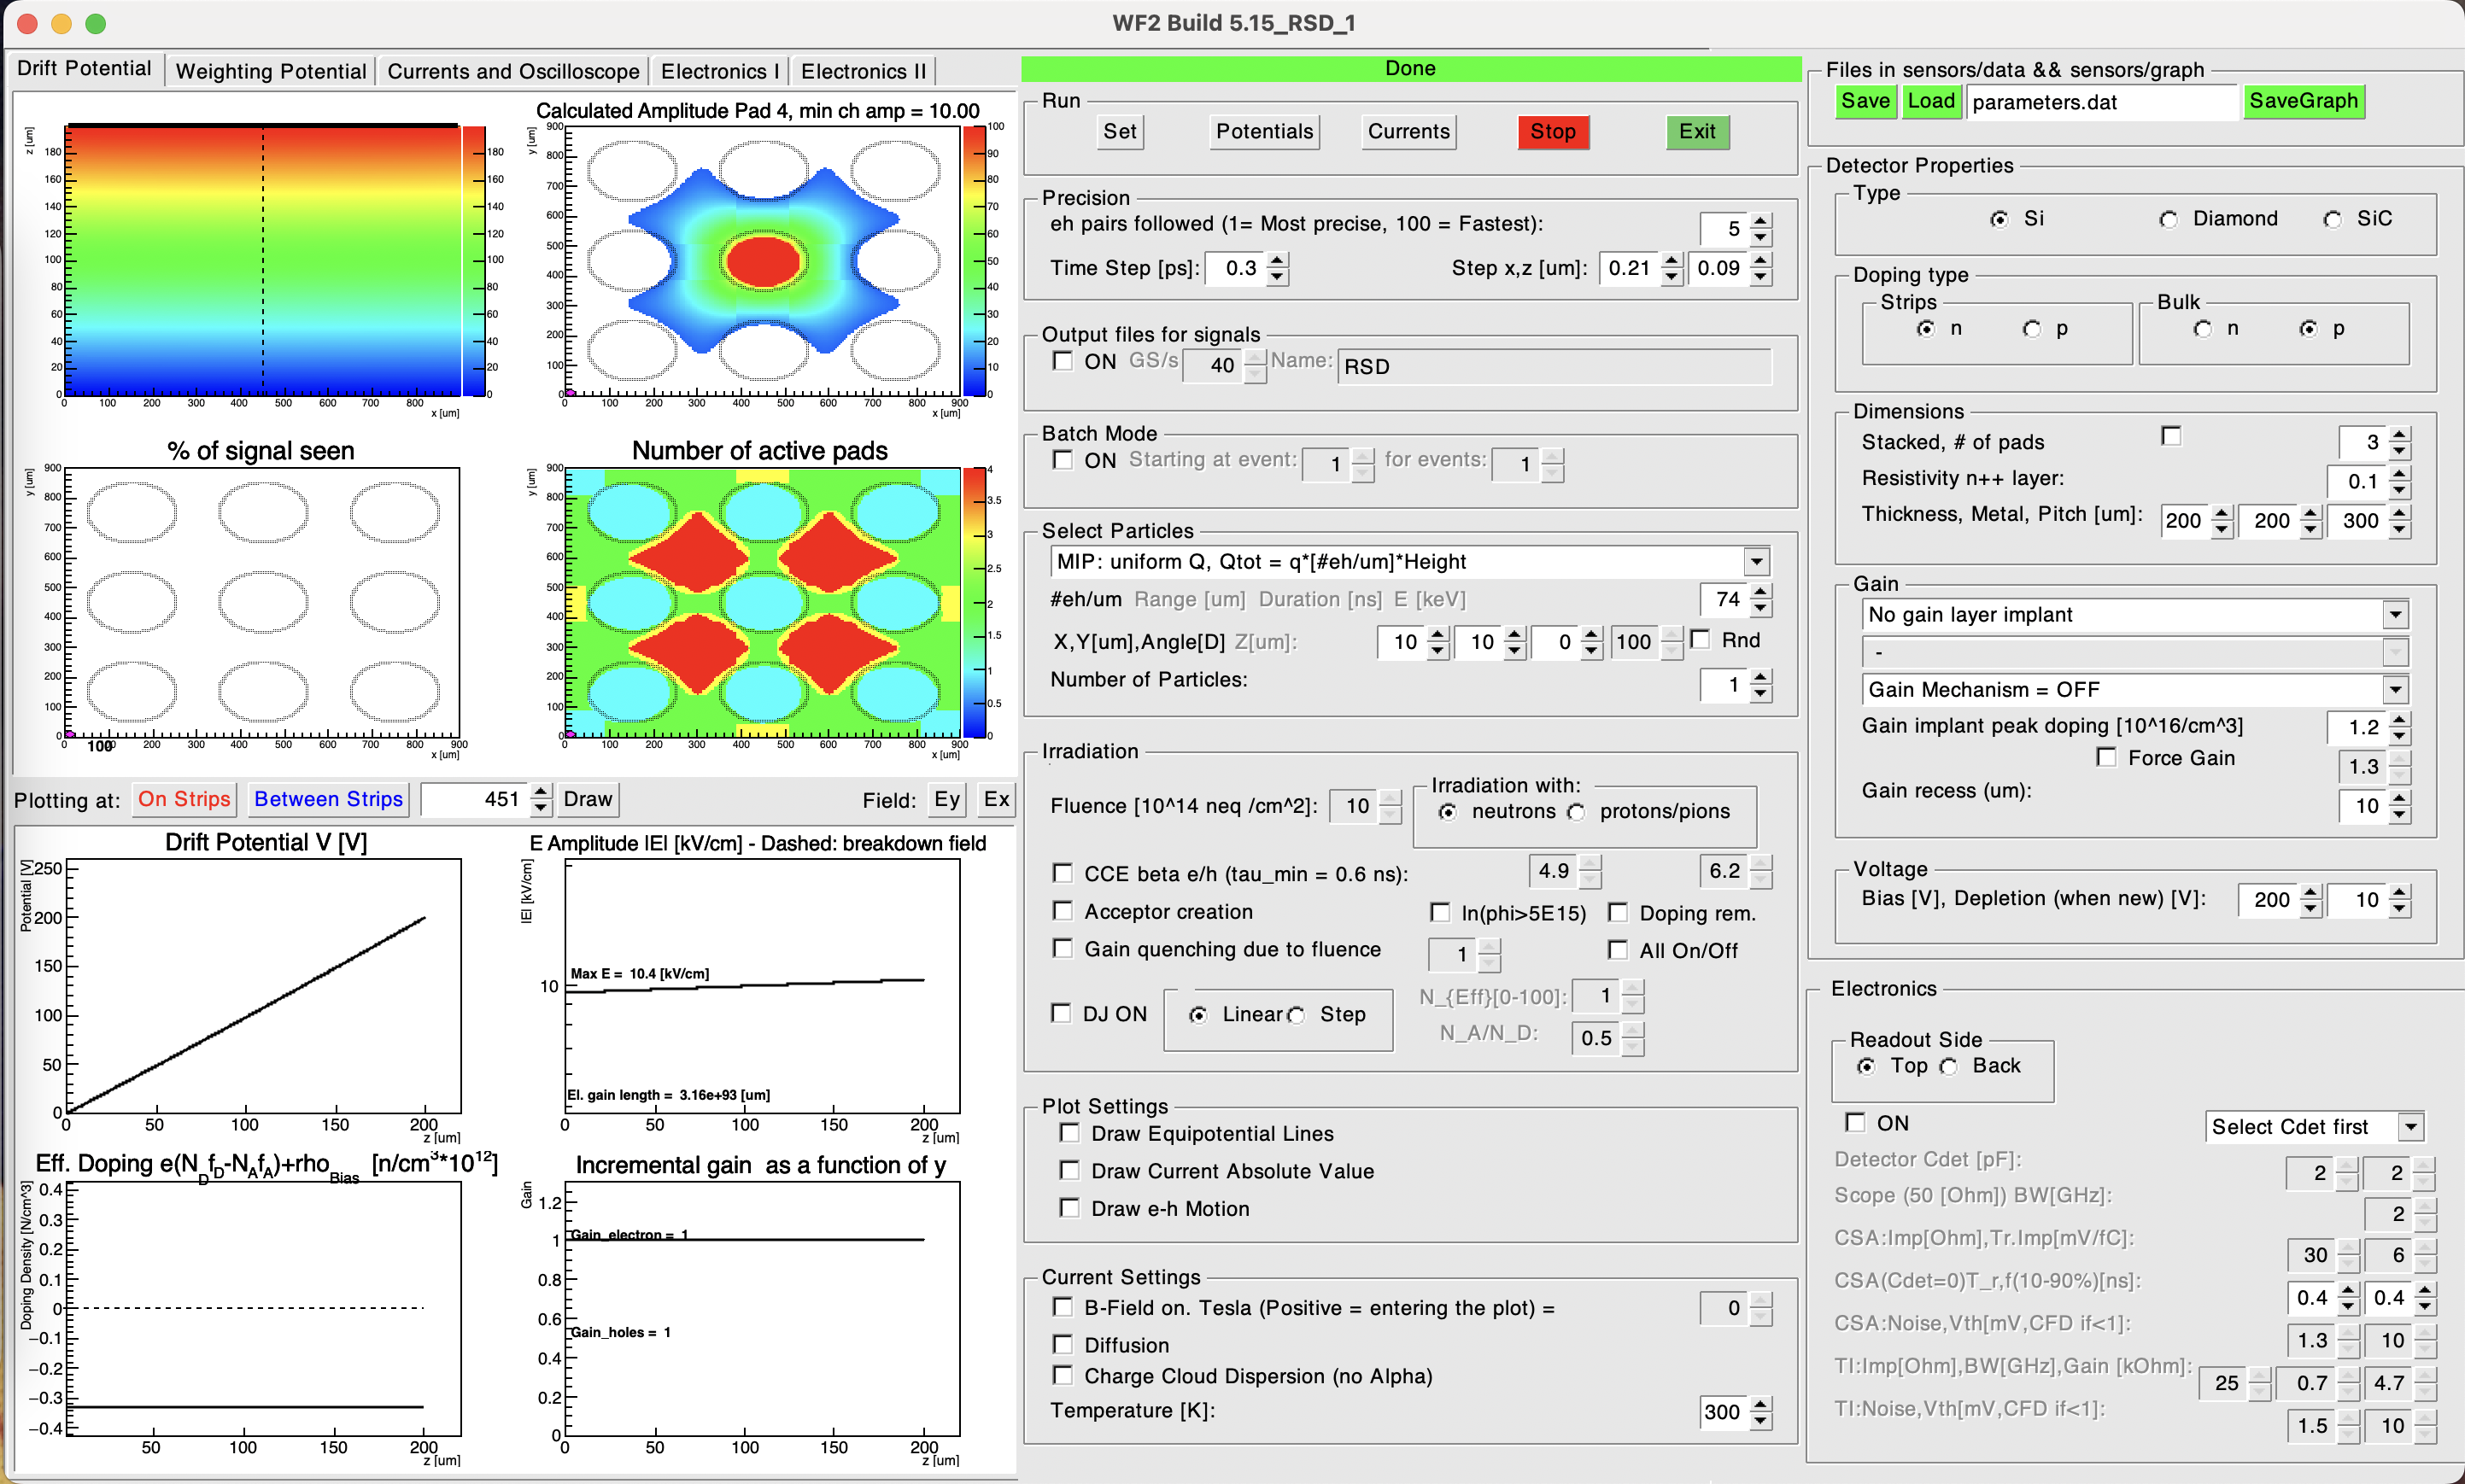
\includegraphics[width=5in]{Images/3x3_pad_structure.png}
            \caption{}
            \label{fig:3x3-pad-field}
        \end{subfigure}%

        \begin{subfigure}[t]{0.99\textwidth}
            \centering
            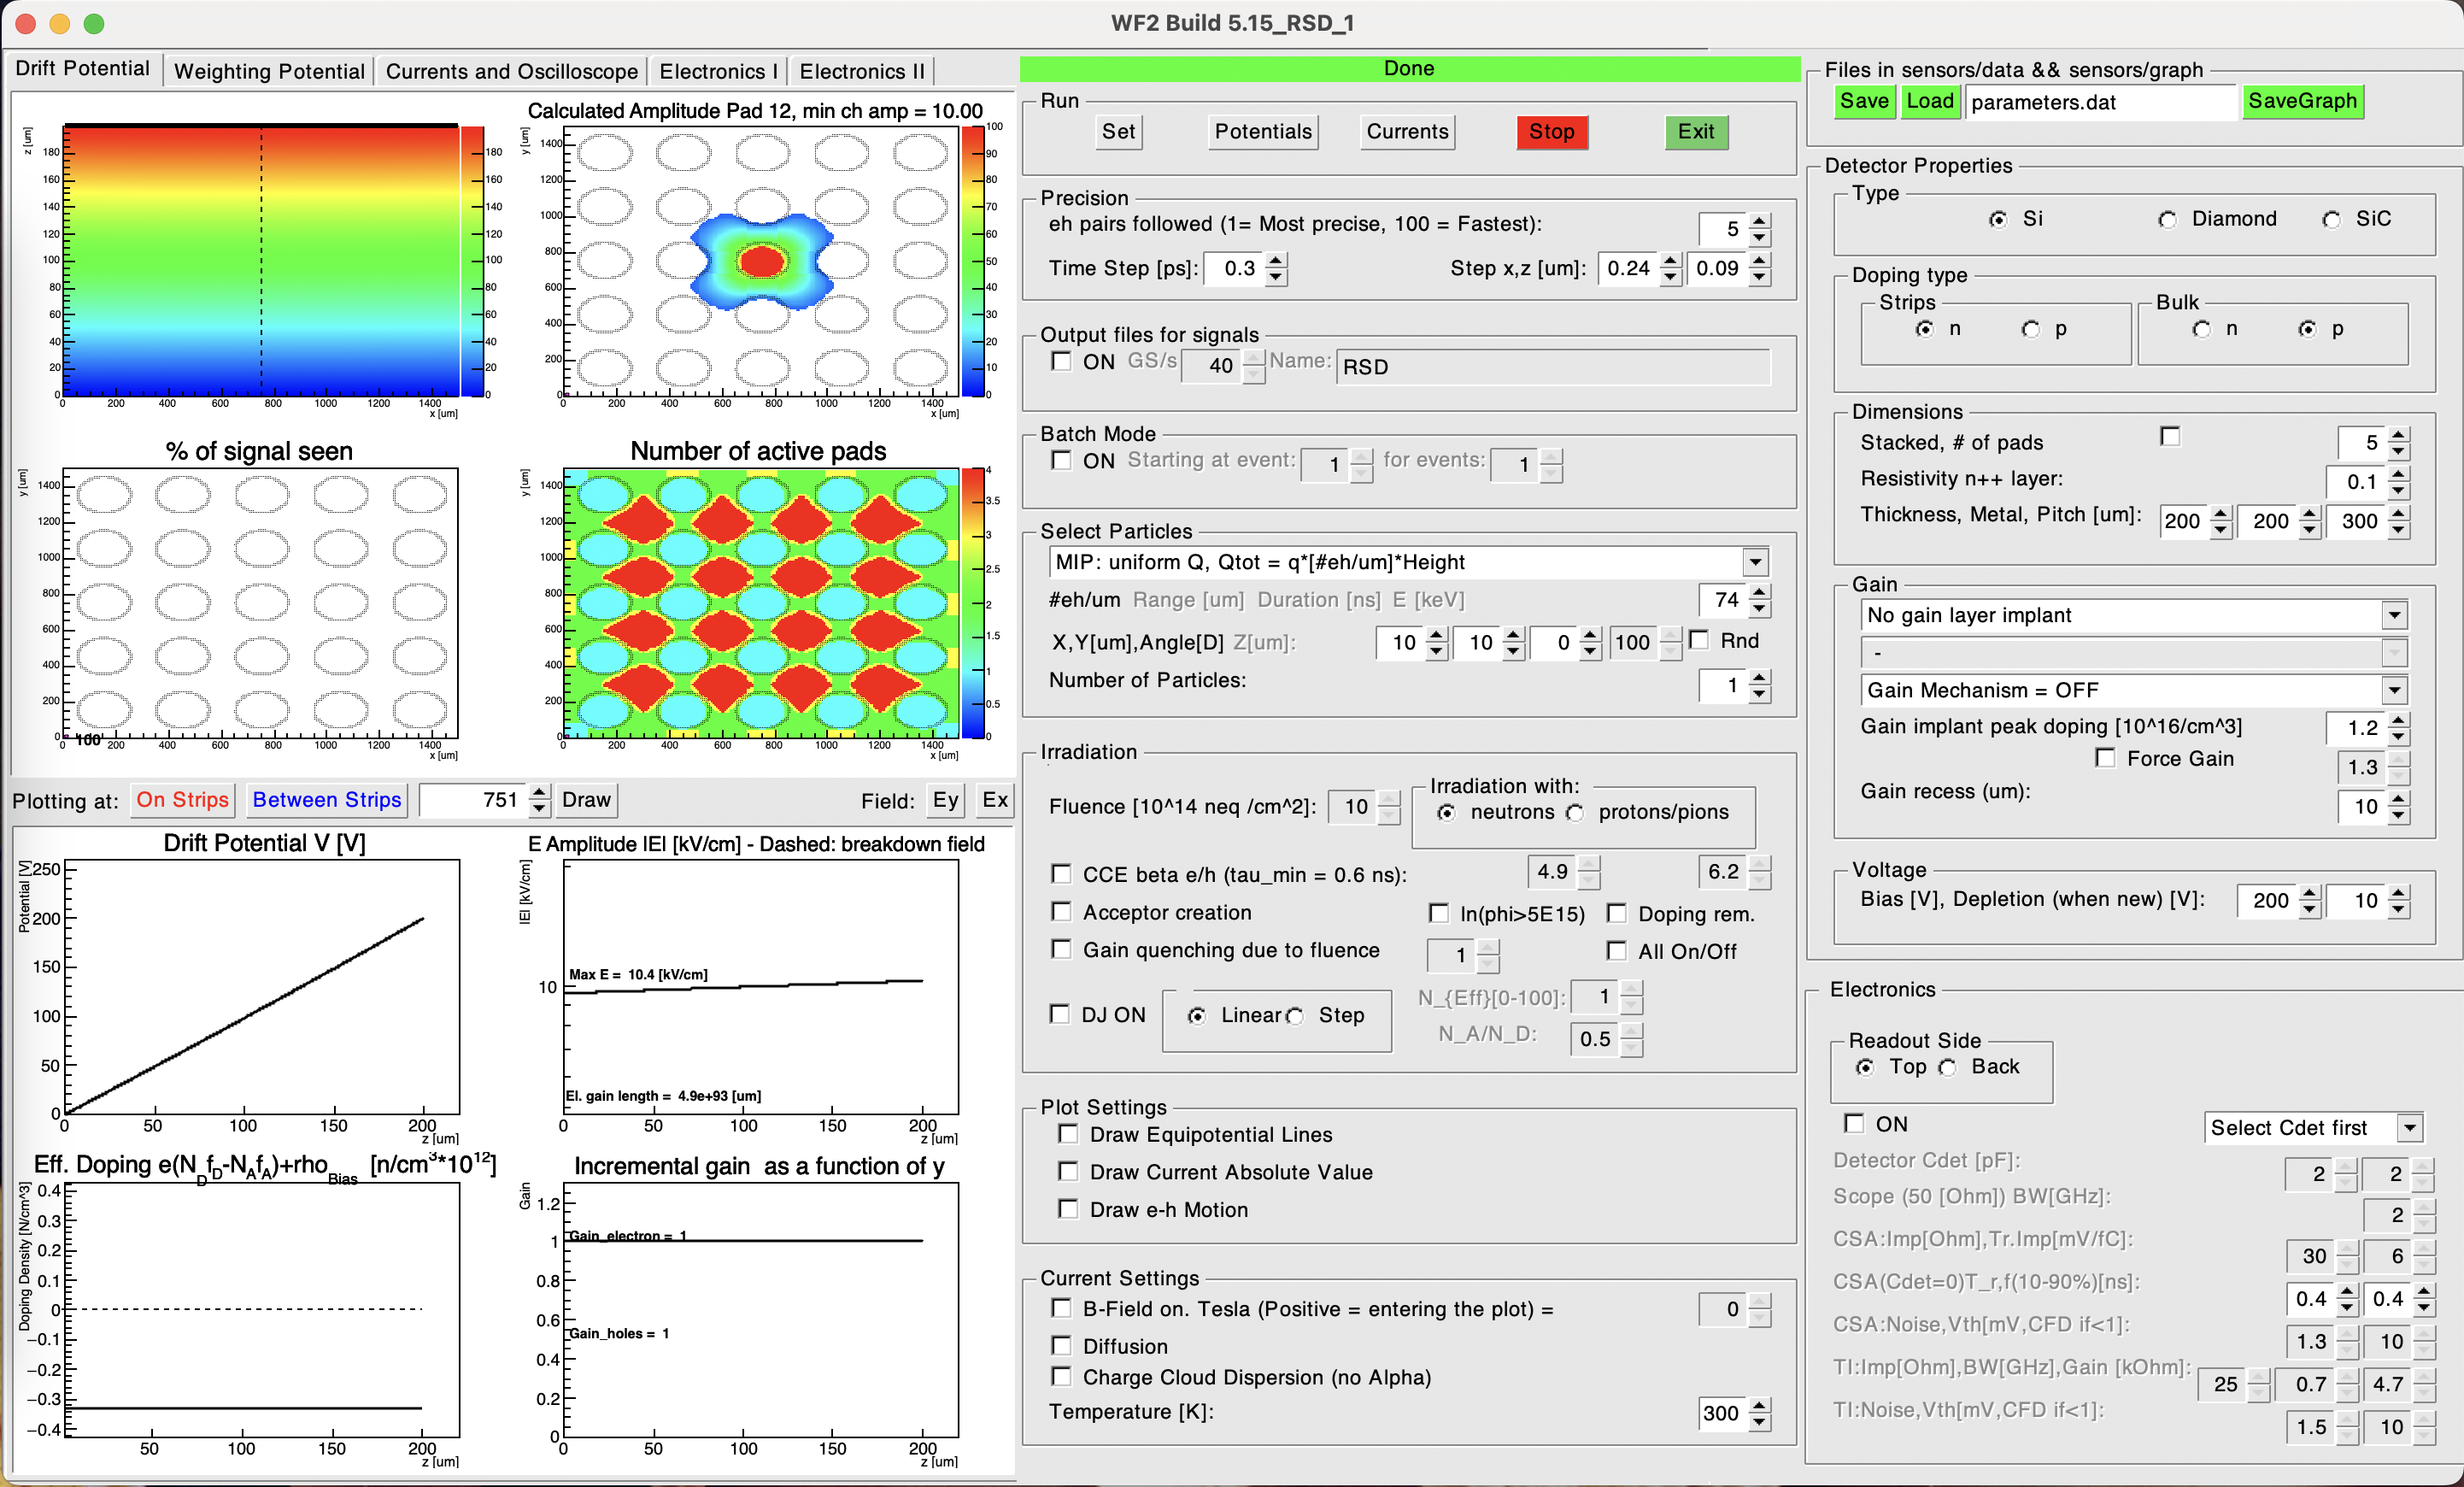
\includegraphics[width=5in]{Images/5x5_pad_structure.png}
            \caption{}
            \label{fig:5x5-pad-field}
        \end{subfigure}
        \caption{Software settings and results for (a) 3 $\times$ 3 and (b) 5 $\times$ 5 pad structures.}
        \label{fig:ss-number-of-pads}
    \end{figure*}
    \item Resistivity n+ layer - Refers to the resistivity of the n+ layer. \hlyellow{Check for changes in current for different resistivity values}. The sheet resistance is 1k$\Omega$/$\square$.
    \item Thickness - The thickness of the detector (if one observes carefully, there is no consideration of pad thickness - which does not affect the potential values under the pads, i.e. in the detector volume). \hlyellow{The value that is assigned to this quantity is the thickness of the bulk substrate (active volume - where the primary charges are created by an incident radiation)}. The top left plot under drift-potential plots is the cross-sectional plot of the electric potential across the detector.
    \item Metal - The diameter of the circular pads (\href{http://personalpages.to.infn.it/~cartigli/Weightfield2/WF2_RSD_files/CERN_Cartiglia_modified.pdf}{Reference} - slide 16).
    \item Pitch - The pitch of the pad geometry. Should be greater than the metal diameter ofcourse.
\end{enumerate}
The options' description for the ``\textbf{Gain}" section:
\begin{enumerate}
    \item Material: Options include Boron, Boron+Carbon, Gallium, and Gallium+Carbon. The addition of Carbon is known to improve radiation hardness \cite{ferrero-radiation-hardness}.
    \item Gain layer - 
        \begin{itemize}
            \item Uniform corresponds to a uniform doping concentration. 
            \item The numbers that follow after the setting/configuration is the position of the electrode from which the gain layer will be implanted. 
            \item LD corresponds to Low-Diffusion [sensors with, say a Boron gain layer that were exposed to a reduced thermal load during production to minimize the diffusion of Boron (Boron low-diffusion)] \cite{ferrero-radiation-hardness}. See \href{https://indico.cern.ch/event/806731/contributions/3516709/attachments/1926118/3188326/191013-VERTEX-RD50-mmoll-acceptor-removal.pdf}{this} link for a better picture.
            \item The number that precedes the configuration refers to the identification tag/name given to the sensor version (Eg - 3.1 refers to the HPK-3.1 sensors made by HPK) \cite{jadhav-sensor-variation, jin-sensor-variation}.
            \item There is one option with the word `Epi': it refers to an Epitaxial substrate. \hlyellow{Although as the setting suggests that the depth of the layer is 3 $\mu$m, but the effective doping plot shows that the layer begins somewhere between 199 $\mu$m and 200 $\mu$m (a small offset is also present for other implant settings).}
        \end{itemize}
    \item Forced gain value - According to Cartiglia's website manual, one can forcefully set a gain value, which in-turn removes the dependance from the bias voltage. A hint along the same direction to what is happening with this step can be understood from Figure 10 in\cite{ferrero-radiation-hardness}.
\end{enumerate}
\begin{table}[!h]
    \centering
    \begin{tabular}{|c|c|c|}
        \hline
        Sensor Version/Name & Thickness & Implant level        \\ \hline
        HPK-1.2             & 35$\mu$m & Shallow (1.1-1.5$\mu$m) \\ \hline
        HPK-3.1             & 50$\mu$m & Deep (1.3-1.9$\mu$m)    \\ \hline
        HPK-3.2             & 50$\mu$m & Deeper (1.9-2.3$\mu$m)    \\ \hline
    \end{tabular}
    \caption{Comparison of some parameters of 3 types of sensors used in WF2-RSD simulations. The numbers in paranthesis in the Implant level column are ones used in WF2-RSD.}
    \label{tab:hpk-sensor-parameters}
\end{table}
\cite{arcidiacono-irradiation} found that the gain layer produced in Low Diffusion (LD-narrower layer profile) is more radiation resistant than the High Diffusion (HD) type; (ii) the co-implantation of carbon in the gain layer volume improves by a factor of $\approx$2 the radiation resistance. \cite{ferrero-radiation-hardness} additionally found that Gallium doping is less radiation resistant than Boron doping, and that narrower gain layer implants are more radiation resistant than wider implants.

Since LGADs have an additional p+ gain layer below the n+ layer when compared with typical silicon detectors, this section contains the options to add this additional layer, define the dopant material, uniformity of doping, choice of physics model for the gain, etc. A brief description of the settings can be found on Cartiglia's \href{http://personalpages.to.infn.it/~cartigli/Weightfield2/Manual_2.html}{WF2 RSD page}.
\newline
The option description for the ``\textbf{Select Particles}" section will follow, but the description has been organised according to the particle type, as each particle type have a different set of options that can be configured. The user has an option to choose from MIPs, X-Rays, Lasers, and a current pulse.
\begin{enumerate}
    \item MIPs - User can define the position at which the MIPs enter, and the number of MIPs. The user can select the type of energy deposition:
    \begin{itemize}
        \item Uniform/Non-uniform energy deposition - User has the option of changing the number of electron-hole pairs deposited per $\mu$m.
        \item Landau - An energy deposition according to the Landau distribution. One can also have a MIP passing through the detector from left to right (Edge MIP Landau), instead the default top to bottom.
    \end{itemize}
    \item Laser - Options can let the user decide if the laser has to enter the detector from top-down, or down-top, or left-right (Edge)
\end{enumerate}
More details on the same can be found in \cite{WF2-incident-particles-cenna}.
\newline
Edge-TCT measurements (shooting laser breams left-right) are used to measure the depletion depth for a certain voltage bias \cite{moll-acceptor-removal}.
\newline
The description of the plots in the ``\textbf{Drift Potential}" section is as follows:
\begin{enumerate}
    \item XZ potential contour (top left) - Contour plot of electric potential across the XZ plane for a Y-plane. \hlyellow{Apparently, since we have uniform doping and a uniform active region, this plot should be same for all Y-values.}
    \item Calculated amplitude plot (top right) for say, pad `A' and minimum charge amplitude = say `B' - Plot across the XY plane that signifies when a particle/radiation passes through a point in that XY-plane, how much of the amplitude reached pad `A'. Signal amplitude below `B' is not considered.
    \item \% of signal seen (bottom left) - For the incident particle(s)/radiation incident at the given position (marked with a purple dot in plot), the percentage amount of the signal reaching nearby pads is represented in this plot. Do \textbf{note} that the percentage value is shown below the pad, and not above it. Sometimes two numbers are displayed outside the plot-area, just poor formatting.
    \item Number of active pads (bottom right) - A plot on the XY-play, such that, for incoming particle(s)/radiation on a certain point in the plot, how many pads will pick up the signal (this number is given by the z-colour-axis).
\end{enumerate}
\newpage
\textbf{Electronics}
Accounting for electronics effect:
\begin{enumerate}
    \item Detector capacitance
    \item Oscilloscope bandwidth
    \item Charge Sensitive Amplifier:
    \begin{itemize}
        \item Input resistance
        \item Rise time/ fall time
        \item Trans-impedance
        \item Noise and threshold voltage
    \end{itemize}
    \item Broad-Band Amplifier (renamed as TI in WF2-RSD):
    \begin{itemize}
        \item Bandwidth and gain
        \item Noise and threshold voltage
    \end{itemize}
\end{enumerate}
Changing parameters of the Charge Sensitive Amplifier (CSA), changes the (Broad-Band) BB amplifier output. This probably suggests that we are looking at a readout `chain' (sensor $\rightarrow$ CSA $\rightarrow$ TI) and not two independent amplifier outputs.
\newline
First, some CAS and TI amplifier parameters were investigated: the noise and threshold voltages (of both CSA and TI) were varied to study what changes they introduce in the final output. A noise voltage of 0.001, 0.1, 1.5, 10, and 50 mV (while other parameters were kept constant) did not show any visible changes in the outputs. The same was done for threshold voltage for 0.001, 0.1, 1, 10, and 50 mV (while other parameters were kept constant) and no visible changes were seen in the output.

subsection{Parameters.dat file}

\section{A full analysis + check of parameters}
\subsection{n+ layer's resistivity}
We look at the effect of resistivity of the n+ layer on the signal characteristic and gain (because \cite{giacomini-lgad} states that doing so changes how much the n+ layer gets depleted).

A conclusive statement on the effect of resistivity on the gain value cannot be made using WF2-RSD, atleast not for the values of resistivity that was used for the study. However, increasing the resistivity showed an elongation of the tail of the second lobe of the signal. This can be explained by the fact that the integral of the signal is 0 (charging and discharging), and the RC value changes for different resistivities.

\begin{figure*}[h!]
    \centering
    \begin{subfigure}[t]{0.49\textwidth}
        \centering
        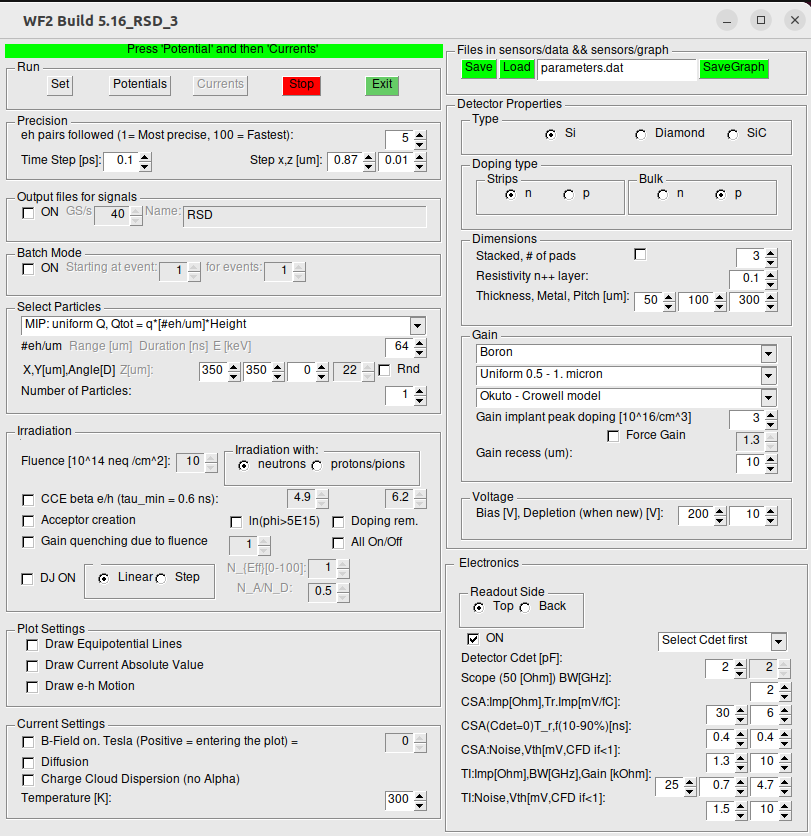
\includegraphics[width=3in]{Images/n_resistivity_other_settings.png}
        \caption{}
        \label{fig:n_resistivity_other_settings}
    \end{subfigure}%
    \begin{subfigure}[t]{0.49\textwidth}
        \centering
        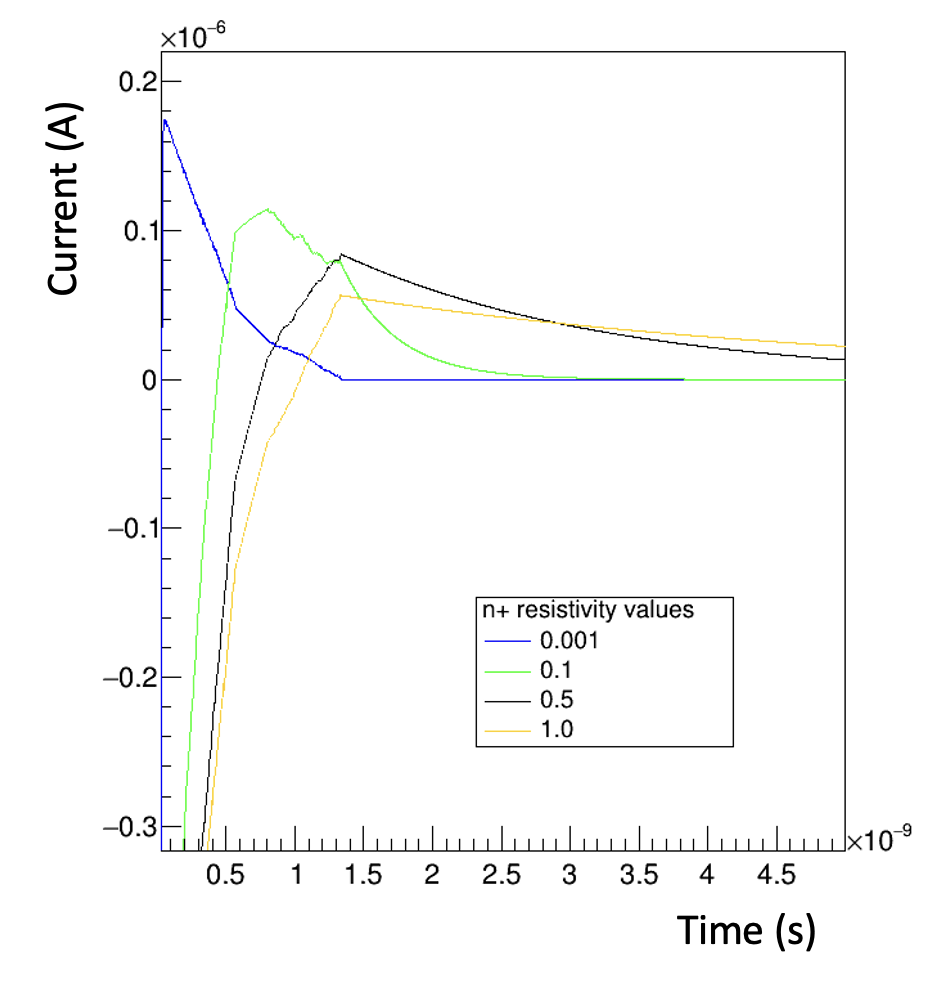
\includegraphics[width=3in]{Images/n_resistivity_plot.png}
        \caption{}
        \label{fig:n_resistivity_plot}
    \end{subfigure}
    \caption{(a) An image of the settings used for the study and (b) the plot of the compiled results obtained as part of this study. As seen, four different values of n+ resistivity was used: 0.001, 0.1, 0.5, and 1.}
\end{figure*}

\hlyellow{The WF2-RSD tool produced a non-intuitive result for resistivity value = 0.0001. The positive part of the signal was much larger than those of the other resistivity values.}

\subsection{Thickness}
Amongst the early silicon sensors (that had no gain layer), the thickness did not affect the amplitude of the signal because of two factors: the number of initial charges produced is proportional to the thickness, and the weighting field is inversely proportional to the thickness. In AC-LGADs however, things are not so simply. It was observed that increasing thickness increases the tail of the first lobe as expected, because the positive charges need to travel a larger distance. \hlyellow{A non-intuitive observation is that the amplitude/height of the first lobe is inversely proportional to the thickness.}

\begin{figure*}[h!]
    \centering
    \begin{subfigure}[t]{0.49\textwidth}
        \centering
        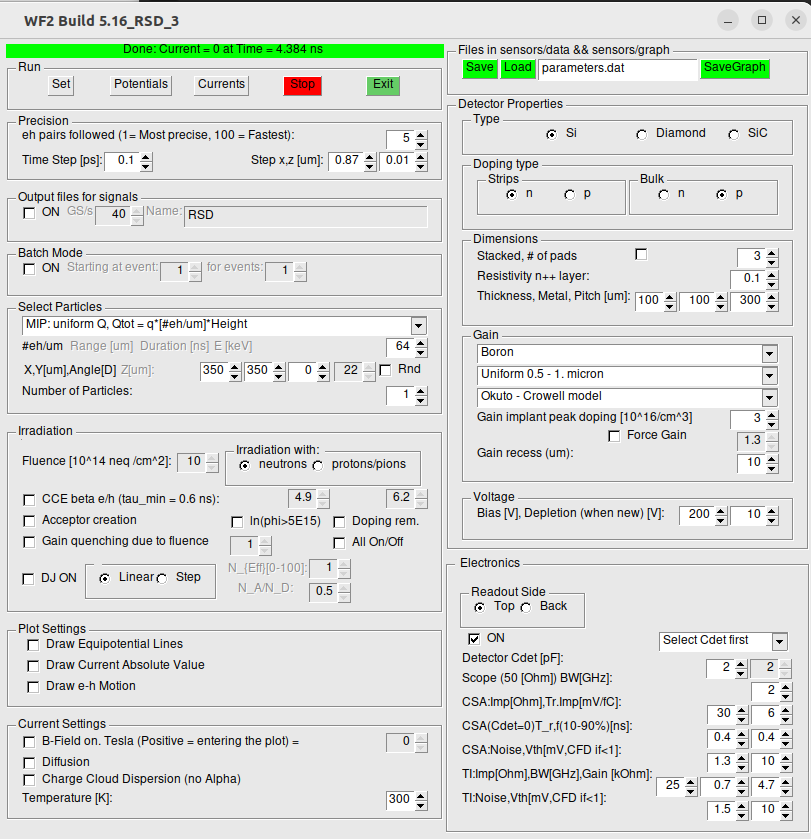
\includegraphics[width=3in]{Images/thickness_other_settings.png}
        \caption{}
        \label{fig:thickness_other_settings}
    \end{subfigure}%
    \begin{subfigure}[t]{0.49\textwidth}
        \centering
        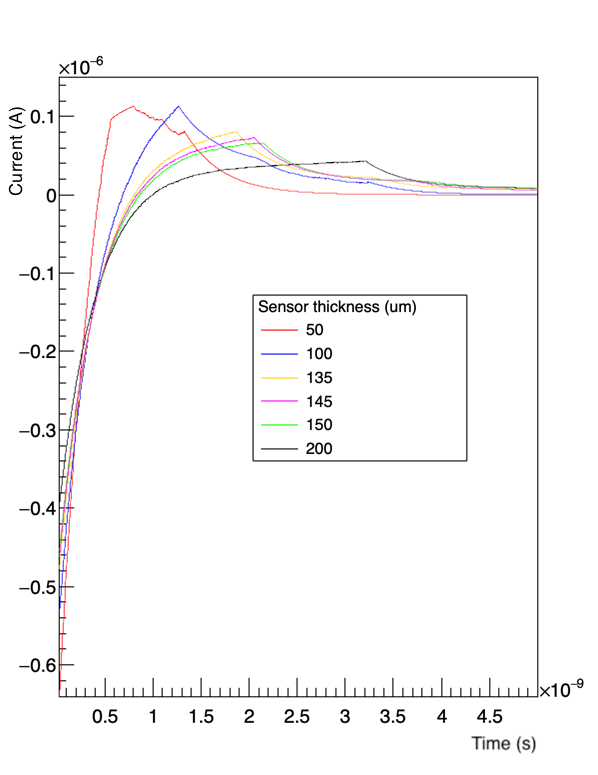
\includegraphics[width=3in]{Images/thickness_plot.png}
        \caption{}
        \label{fig:thickness_plot}
    \end{subfigure}
    \caption{(a) An image of the settings used for the study and (b) the plot of the compiled results obtained as part of this study. As seen, four different values of thicknesses was used: 50, 100, 135, 145, 150, and 200 $\mu$m.}
\end{figure*}

The reason for looking at 135 $\mu$m and 145 $\mu$m is that alongwith thickness, there was a parallel study on the maximum electric field's variation with thickness. There seems to be a numerical fluctuation (probably due to mesh-effects) of the maximum field value around 150 $\mu$m.

\subsection{Time delay from hit position}
Depending on where the incident particle hits the sensor, there is a time delay introduced for the signal to reach the electronics. This comes from the time charges takes to reach the electrode, or more specifically, the wirebond. Madrid, C. in his large AC-LGAD paper reported that for different hit positions on the strip the time delay increases as one goes away from the wirebond. Simulations were done for pad diameters (200, 300, 400, and 450 $\mu$m) and varying y-coordinates (100, 150, 200, 250, and 600 $\mu$m) for the same x-coordinate (20$\mu$m away from the end of the pad). In WF2, the current and electronic response of a sensor was simulated for different hit positions (in the gap region) and no conclusive correlation between the time when the current hits 0A, and distance from the center of the pads, was found. This statement could atleast be made only for the geometries that was tried. This could be because the strips that displayed this result in the above stated paper were of larger order of lengths, so this effect might not be prominent in smaller pad sizes.

\begin{figure*}[h!]
    \centering
    \begin{subfigure}[t]{0.49\textwidth}
        \centering
        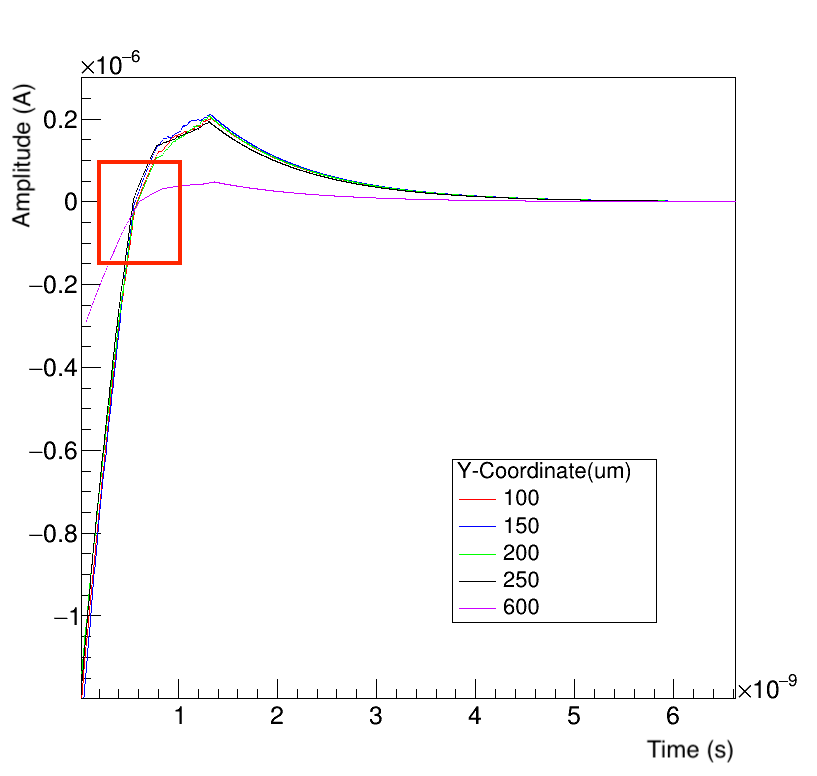
\includegraphics[width=3in]{Images/time_delay_plot_200W_full.png}
        \caption{}
        \label{fig:time_delay_plot_full}
    \end{subfigure}%
    \begin{subfigure}[t]{0.49\textwidth}
        \centering
        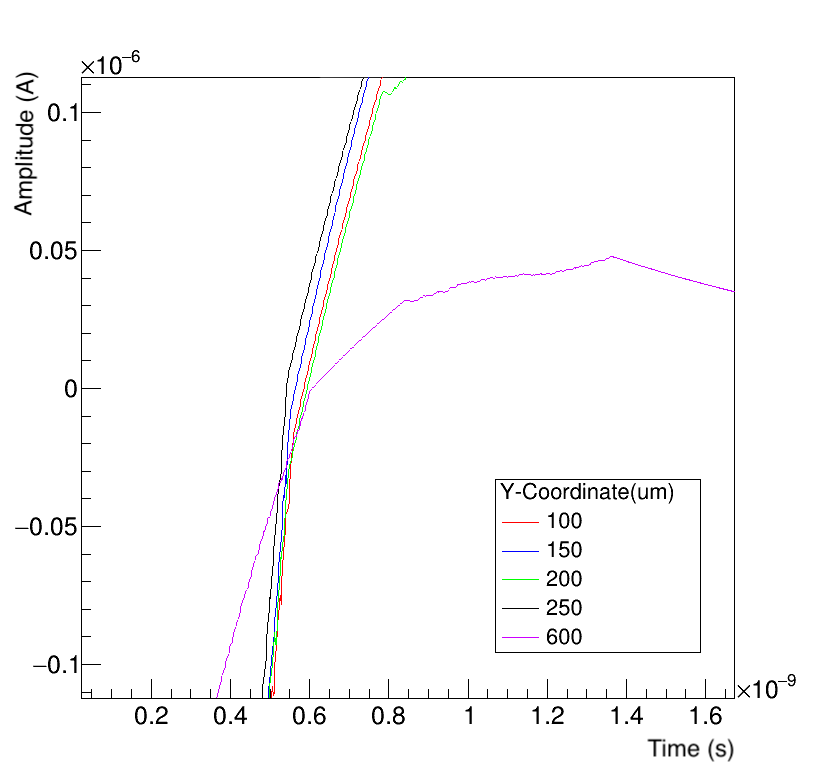
\includegraphics[width=3in]{Images/time_delay_plot_200W_sig.png}
        \caption{}
        \label{fig:time_delay_plot_sig}
    \end{subfigure}
    \caption{A plot of the signals from a sensor with 50 um thickness, 500 um pitch, 200 um pad width for different incident hit positions (same x-coordinate, but different y-coordinates) in the gap region. The red box in Figure (a) corresponds to the region enlarged to produce Figure (b)).}
\end{figure*}

\subsection{Changes introduced in different versions}
WF2\_5.4 has another update with regard to choosing AC/DC coupling on the top-readout surface, a feature that WF2\_5.17 does not have. Additionally, some other physics models for the gain layer (which is called as ``gain parameterisation'' in Cartiglia's website) seem to have been added.
\newline
That said, WF2-RSD does not have the option to introduced AC-coupling in the readout, so can we not fully simulate AC-LGADs? According to one of Cartiglia's \href{https://indico.cern.ch/event/928957/contributions/3913535/attachments/2069369/3473666/FCCee_Cartiglia.pdf}{slides}, it seems like WF2-RSD is for AC coupled simulations by default.
\newline
I still have not deeply looked at the differences in WF2-RSD between version 5.15 and version 5.16.

\bibliography{references}

\end{document}